\documentclass[12pt]{article}
\usepackage{natbib}
\usepackage{graphicx}
\usepackage{float}
\usepackage[hyphenbreaks]{breakurl}
\usepackage[hyphens]{url}
\usepackage{listings}


\usepackage{listings}
\usepackage{xcolor}

\definecolor{dkgreen}{rgb}{0,0.6,0}
\definecolor{gray}{rgb}{0.5,0.5,0.5}
\definecolor{mauve}{rgb}{0.58,0,0.82}

\lstdefinestyle{myScalastyle}{
  frame=tb,
  language=scala,
  aboveskip=3mm,
  belowskip=3mm,
  showstringspaces=false,
  columns=flexible,
  basicstyle={\small\ttfamily},
  numbers=none,
  numberstyle=\tiny\color{gray},
  keywordstyle=\color{blue},
  commentstyle=\color{dkgreen},
  stringstyle=\color{mauve},
  frame=single,
  breaklines=true,
  breakatwhitespace=true,
  tabsize=3,
}



%Gummi|065|=)
\title{\textbf{ID2203 Project}}
\author{Max Meldrum\\
	Vaikunth Srinivasan A}
\date{\today}
\begin{document}

\maketitle

\section{Introduction}
In this project, we implemented a distributed in memory key-value store with linearizable operation semantics. We take advantage of the Kompics \cite{DBLP:conf/p2p/AradDH09} programming model and utilise the Kompics Scala DSL. We were given a lot of freedom when it came to the design of the system, as long as we satisfied linearizability. We had the option of either building the entire system from scratch or using an existing project template\footnote{https://gits-15.sys.kth.se/lkroll/id2203project18scala} that sets up the basic features such as single-partitioning, overlay and routing. It was an easy choice, we went with the template. Our implementation is hosted on github\footnote{https://github.com/Max-Meldrum/id2203-project}

\section{Infrastructure}
In this section, we describe how our system is designed.

\subsection{Overview}

The key-value store is portioned based on the key-space with each partition responsible for a particular key range. The partitions constitute a replication group i.e., each partition consists of a primary and its replicas. The replication groups are responsible for handling client requests and providing linearizable operation semantics.
\begin{figure}[H]
  \centering
  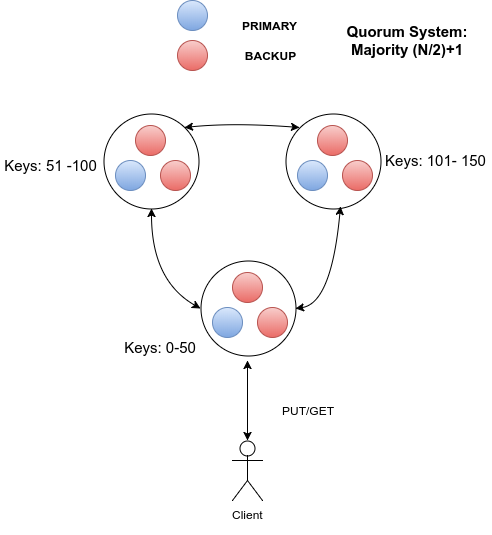
\includegraphics[scale=0.6,clip]{img/architecture}
  \caption[Caption for LOF]{System architecture}  
  \label{fig:picture}
\end{figure} 

\subsection{Partitioning}
As one of the requirements was that the system should be able to support a partitioned key-space, we have opted to go for range-partitioned integers. These partitions are distributed over the available nodes. Each partition is considered to be a replication group and we use passive replication where each of these groups consist of one primary and multiple backups. The replication within a group is done with respect to a specific replication degree.

\subsection{System Model}
We decided to go for the fail-silent model, where we assume our environment to be asynchronous. To ensure consistency across all replicas in a certain replication group, we use a primary-backup scheme and implement an Atomic Broadcast protocol that is heavily inspired by Zab \cite{Junqueira:2011:ZHB:2056308.2056409} which ZooKeeper \cite{Hunt:2010:ZWC:1855840.1855851} relies on.

\subsubsection{Assumptions}
We are assuming that all our network based components have access to a perfect-link abstraction.

\section{Replication Protocol}

\subsection{Atomic Broadcast}
Zab, which is the algorithm behind ZooKeeper, is a crash-recovery atomic broadcast algorithm. A primary server handles client requests and broadcast state changes to the rest of the backups. The delivery order of state updates is crucial. This order is often referred as Primary Order \cite{Junqueira:2011:ZHB:2056308.2056409}. Zab consists of 3 phases. However, as we are not implementing our kv-store in a crash-recovery model, we skip the synchronising phase and only implement Leader Activation and Active Messaging \cite{zk-internals}.
\newline{}\newline{}
In this report, we will put more focus on describing on how the broadcast phase works and not so much on Leader Activation. Zab assumes all communication channels are FIFO (TCP), by utilising FIFO channels, preserving the ordering guarantees becomes very easy \cite{Reed:2008:STO:1529974.1529978}. This was not an issue for us as the channels in Kompics provide FIFO semantics. The Active Messaging in Zab is very similar to a classic two-phase commit.  Once a primary has received a client request, it broadcasts out proposals that includes its monotonically unique proposal id. Replica’s that receive proposals return with an acknowledgement (ACK). As soon as the primary has received a majority of ACKs for a given proposal, it will issue a commit to itself and its backups. This whole process can be seen in figure 2 down below.


\begin{figure}[H]
  \centering
  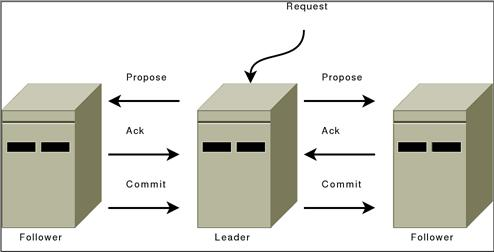
\includegraphics[scale=0.90]{img/2pc.jpg}
  \caption[Caption for LOF]{ZooKeeper messaging \protect \cite{zk-internals}}  
  \label{fig:picture}
\end{figure}


\subsection{Failure Detection}
As we are in the fail-silent model, we do not rely on a perfect failure detector or an eventually perfect failure detector. We utilise the Zab approach, where the primary periodically checks if it has a majority of replicas connected to it. This means that backups frequently send heartbeats to the primary. If a primary notices that it no longer has a majority of followers connected, it enters an election phase. What if backup’s are isolated and cannot connect with anyone? The solution to this is that backup’s also receives heartbeats from the primary. If a backup stops hearing from the primary, it will enter an election phase and attempt to elect a new primary.

\subsection{Leader Election}
As mentioned in \cite{zk-internals}, the only requirements that we have to meet is that the leader has seen the highest (epoch, commitNumber) and that a majority of replicas has committed to following it. Our leader election is not an optimal approach, but it satisfies the previous mentioned requirements. Once a replica enters election phase, it broadcasts a NewLeaderProposal event. Replicas receiving the proposal compare the commitNumber and epoch to its own, if it is safe, then we reply with a NewLeaderAck. After acquiring a majority, a NewLeaderCommit is sent out and the replica enters the Primary state and is now able to execute client requests.

\section{Kompics Components}
\subsection{Overview}
\begin{figure}[H]
  \centering
  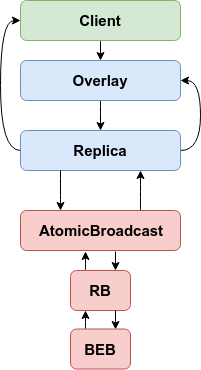
\includegraphics[scale=0.90]{img/components.png}
  \caption[Caption for LOF]{Component Structure}  
  \label{fig:picture}
\end{figure}
In figure 3, we show the relationships between the most important Kompics components in our system. The client initially connects with a bootstrap server, it then forwards it request to an overlay which checks if the which partition should be handling the request. If the current server is in the group, the overlay forwards the request to the Replica component. If the current node is not involved with the partition, it routes the request to any of the nodes in the replication group responsible for the partition.

\subsection{Replica}
As most of the logic happens in the Replica component, it will be the only component we look further into.
\newline{}\newline{}
The Replica starts of with an InActive state, later when it is has been fully activated, it can take the role of either Primary, Backup or Election. To enable replica's to send heartbeats, we utilise Timers. Primary and backups have separate timer id's. If a backup changes state to Primary, it then cancels the backup timers and enables primaries. Same goes for the other way around. We earlier discussed in 3.1 and 3.3 how we deal with Atomic Broadcast and Leader Election, now lets look at how it relates to the KompicsEvent's that each Replica can send and receive.
\newline{}\newline{}
Atomic Broadcast KompicsEvents:
\begin{lstlisting}[style=myScalastyle]
case class AtomicBroadcastProposal(clientSrc: NetAddress, epoch: Int, proposalId: Int, event: KompicsEvent, addresses: List[NetAddress]) extends KompicsEvent with Serializable {
  val uuid: UUID = UUID.randomUUID()
}
case class AtomicBroadcastAck(src: NetAddress, dest: NetAddress, event: KompicsEvent) extends KompicsEvent with Serializable
case class AtomicBroadcastCommit(payload: KompicsEvent) extends KompicsEvent with Serializable

\end{lstlisting}
Leader Election KompicsEvents:
\begin{lstlisting}[style=myScalastyle]
case class NewLeaderProposal(src: NetAddress, epoch: Int, lastCommit: Int, group: Set[NetAddress]) extends KompicsEvent with Serializable

case class NewLeaderAck(src: NetAddress, dest: NetAddress, event: KompicsEvent) extends KompicsEvent with Serializable
case class NewLeaderCommit(payload: KompicsEvent) extends KompicsEvent with Serializable
\end{lstlisting}

\section{Testing}
Here, the Kompics Simulation framework has been used for testing and verifying various properties by simulating a scenario related to their specifications. A test package consists of a test scenario and a respective client to test the operations on the server. These scenarios are a good indication of whether the implementation is correct or not.

\subsection{Operations}
The capability of the store to support the fundamental operations such as GET, PUT and CAS is tested here with a scenario which is designed to start a cluster of servers as well as a test client. The client issues a set of PUT operations which are followed by a set of GET operations to read the values stored at the corresponding keys after the PUT operation. And subsequently, a set of CAS operations passing the parameters key, value and reference value is executed. During the CAS (Compare and swap) operation, the previously read value is compared with the current value and if there is a match, the swap occurs with the new value. Upon the termination of this test, we could verify that all operations were successfully executed and expected responses were received.

\subsection{Linearizability}
Linearizability is a correctness condition for concurrent objects that exploits the semantics of abstract data-types. In a linearizable system, every operation seems to execute atomically and instantaneously at some point between its invocation and response. The test for linearizability is implemented as follows: we consider a scenario where a set of servers is started as a cluster along with their corresponding sequential client. The test scenario basically takes as an input a sequential specification and a concurrent history of the operations which are written into a queue. A decision procedure then checks whether the history is linearizable with respect to the specifications. 

\section{Leader Lease}
When a replica enters the Primary state and the lease option is on, a LeaseRequest is broadcasted to all servers. Once it the primary has gotten a majority of LeasePromise's, it enables the so called fast-read mode. As long as \(C(T) - tL < 10*(1-p)\) is satisfied, it can serve GET requests without contacting a majority of replicas. Important thing to note is that we do not use a real clock drift rate, we simulate it with a randomised rate between 0.1-0.2.
\newline{}\newline{}
We did not write test scenarios that interleave reads with writes during a partition. The reason for this is that our implementation is different than Sequence-Paxos/Multi-Paxos in the sense that when a primary is isolated from the rest of the cluster, it will no longer be in contact with a majority of replicas. Hence, GET requests wouldn't be allowed as the replica has entered an election phase. The benchmark was performed by inspecting the real-time of the simulation.
\begin{figure}[H]
  \centering
  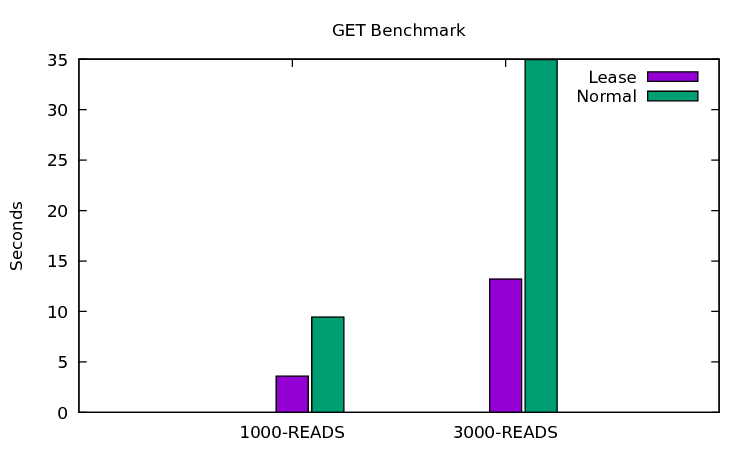
\includegraphics[scale=0.5]{img/benchmark.png}
  \caption[Caption for LOF]{Leader Lease enhancement}  
  \label{fig:picture}
\end{figure}

\section{Contributions}

\begin{itemize}
	\item{Max Meldrum\newline{}\newline{}Replication protocol, Infrastructure and Broadcast}
	\item{Vaikunth Srinivasan A\newline{}\newline{}Broadcast and Testing}

\end{itemize}
\bibliography{references}
\bibliographystyle{unsrt}


\end{document}
